% Separated from the main body of my notes since 
% this topic has appeared several times elsewhere
 
\section{Theoretical orientation}\label{sec:theoretical-orientation}

{\small

\subsection{Constituency and dependency relations}

In a word, the theoretical framework of this note 
is \ac{blt}\citep{dixon2009basic1,dixon2010basic2,dixon2012basic3}
with generative flavors.
Here by \term{generative} I mean 
Minimalism plus Distributed Morphology plus Syntactic Cartography 
(but the Antisymmetry theory is not strictly followed here; 
I only use the idea of a semi-rigid template of functional projections).
Although generativism is harshly criticized by Dixon, 
I believe this is largely due to notational reasons;
some criticisms, like ``generativism sticks to the universal notation of words''
or ``generativists blindly believe in a 
noun-verb distinction \emph{exactly} the same as English'',
are invalid in the aforementioned framework. 
To connect the aforementioned school of generativism and \ac{blt}, 
I list some observations:
\begin{itemize}
    \item First, note that ``functional heads'' are just 
        an alternative way to say ``grammatical categories'' or ``grammatical relations''
        in a constituency-based framework doing away with dependency relations.
        The constituency-dependency correspondence 
        has long been discovered 
        \citep{schneider1998linguistic,osborne2011bare,kahane2015syntactic,nefdt2023notational}. 
        On the other hand, 
        ``lexical heads'' -- nouns, verbs, etc. -- 
        lie at the \emph{bottom} of an ``extended \ac{np}'' (i.e. the DP projections) 
        or an ``extended \ac{vp}'' (i.e. the CP projections).
        This settles the issue raised by many descriptive linguists: 
        the term \term{head} is no longer used in the same way 
        as it was in contemporary generativism.
        The \term{head} of descriptive linguists is essentially the \term{root} in Distributed Morphology.
    \item It's possible to ``compress'' the Minimalist constituency (or dependency) structure: 
        removing invisible functional projections, 
        replacing labels like SpecTP with ``subject'',
        using the term \term{head} to refer to the lexical head, etc.
        Thus, we are able to automatically 
        obtain more traditional constituency analysis (as in \citet{cgel})
        or dependency analysis 
        from generative trees. 
        The counterpart of c-command relations in the dependency analysis 
        is how ``tight'' a dependency relation is:
        that the relation between the verb and the object is tighter 
        than the relation between the verb and the subject 
        is equivalent to that the subject has a higher position in the syntactic tree.
    \item One implicit message hidden in the idea that 
        \acs{np}s and clauses are the only two types of constituents 
        in \citet{dixon2009basic1}  
        is that when we finish building up an \acs{np} 
        and insert it into an argument slot in a clause, 
        the syntactic processing enters a new stage;
        on the other hand, the difference between a half-finished \acs{np}
        and a completely finished \acs{np}
        is not that huge.
        Now if we use constituency analysis all the way down, 
        we are in the risk of losing this piece of information.
        This is settled by the concept of \emph{phase} in modern generativism:
        when typologists argue for recognizing only noun phrases and clauses as constituents, 
        they are essentially referring to phases. 
    \item The phase theory also explains why some have the intuition that 
        the \term{verb phrase} should exclude the object: 
        because when the CP is being built, 
        the arguments are already ``frozen'', 
        and what are manipulated and realized together 
        are verbal functional heads -- that's exactly \emph{their} verb phrase. 
        The similar thing happens for a \term{word} (see the next point). 
    \item Some people (many functionalists, but also some formal grammarians) 
        really don't like the idea that 
        differences in constituent order have their roots in 
        the constituent structure and especially in movements. 
        They say constituent order \emph{directly} reflects 
        grammatical relations and categories like topicalization, 
        instead of the mainstream generative idea that 
        constituent order reflects constituency relations,
        which then codes things like topicalization. 
        The exact meaning of ``directly reflect'' however is rather hard to tell 
        from an empirical perspective.
        What we already know is that
        quantitative researches suggest that 
        at least a semi-configurational approach 
        (i.e. a linear template with fixed constituent slots in it)
        is needed to fully capture Latin constituent order, 
        because the diachronic change of the frequency of OVAux
        looks very different from the diachronic change of the overall OV frequency,
        which includes, say, OAuxV \citep{danckaert2015studying}.
        But after we accept the semi-configurational approach, 
        we can then do tests like, say, Principles A, B, and C, 
        coordination and ellipsis tests, etc.,
        on slots of these templates, 
        and usually a hierarchy of 
        relative ``strength '' of dependency relations
        can be established 
        \citep[\citesec{1.6}]{danckaert2017development}.
        Then, by the duality between constituency and dependency, 
        usually we will find 
        that a constituency-based analysis is \emph{accurate} for 
        a so-called non-configurational language, 
        although it may not be \emph{convenient} 
        for its documentation.
    \item Finally, the hierarchy of functional heads -- or in other words, 
        grammatical relations and categories -- 
        can be ``routinized'' and packaged,
        and how they are stored in the actual brain 
        may have more resemblance to \ac{tag}. 
        Most inflection patterns, for example, 
        seem to be packaged, 
        which explains why sometimes they seem to be psychologically different from syntax, 
        though Distributed Morphology has shown it's possible to treat the grammar 
        as syntax all the way down. 
        This is just what people call \term{construction}.
        However, it seems a construction is still not a packaged \emph{linear} sequence: 
        its inner structure still observes the usual rules for syntax 
        and may (although of course sometimes may not) engage 
        actively with productive syntactic elements. 
        Thus a structuralist -- as opposed to canonical constructivism -- 
        analysis is still valuable.
        Note that the adoption of functional hierarchy à la Cinque 
        also means the distinction between adjuncts and complements/specifiers 
        is eliminated, 
        and the argument-adjunct distinction then becomes epiphenomenal 
        and is no longer a primitive concept in grammar:
        like the concept of subject, 
        argumenthood of a clausal dependent 
        is now defined by a collection of more primitive properties, 
        each of which may assume cross-linguistic variation
        \citep{mcinnerney2022argument}.
        A clausal dependent position may be defined as an argument 
        because of semantic reasons,
        or because of the verb root can't be realized 
        without the existence of that clausal dependent
        \citep[\citechap{9}]{siddiqi2009syntax},
        or because of its base position is lower than what is traditionally 
        known as adjuncts.
        Of course, the general tendency is to identify all the three criteria,
        but corner cases like 
        that one semantic argument is syntactically omitted
        or that an applicative device regularly
        attaches an optional argument to the core argument structure
        happens all the time; 
        worrying too much about the argument-adjunct distinction 
        (or similar issues) is probably not wise.
\end{itemize}

\subsection{The word}

\subsubsection{Wordhood}

Three criteria are involved in wordhood determination -- 
or, to be more accurate, what people call words,
since as we are going to see, 
although each of the definition of wordhood 
seems to have its status in the grammar cross-linguistically,
we shouldn't expect there to be any strong implicational relation 
among the three types of wordhood.

\paragraph{Three definitions of wordhood} The three criteria are: 
syntactic status as a mini-constituent 
(although how small they should be is not without controversy: 
usually we say grammatical relations realized as compounding or affixation 
are word-level relations, 
but this definition is already influenced by 
intuition from morphological and phonological wordhood);
realizational (or ``post-syntactic'') morphological  status 
as a unit with a fixed template;
status as a phonological unit surrounded with word boundaries.

In the first definition, a word is just a mini-phrase 
(in the above phase-as-descriptivist-phrase sense, 
possibly a mini-tree, possibly a collective realization of a span of functional heads).
The syntax all the way down analysis taken in this note 
therefore explains why we always have controversies 
concerning whether a unit is a word or a phrase 
(like \form{American history teacher} 
-- note that its inner parts don't actively participate in other syntactic processes):
this is no objective standard for drawing a line between the two. 
What are objective are the morphosyntactic units recognized: 
\form{American history teacher} is a nominal compounding structure 
(a certain kind of FP below the NumP projection),
regardless of whether you say it's a word. 

The first definition of wordhood largely overlooks 
case or \acs{tame} affixes:
they are technically categories within the \acs{np} or the clause, 
and not categories within the syntactic word.
In other words it is about the difference 
between, say, nominal derivation and modification in the noun phrase.
The morphological definition, on the other hand, 
is about how functional items are realized, 
or in other words, it's about the distinction 
between the affix and the auxiliary.
We can say it's more about inflection.

According to Cartography syntax, 
cross-linguistically, 
we should find similar patterns of functional heads,
so we should expect to see a morphosyntactic unit 
of a size similar to what we usually call words in English 
in another language, 
although the native speakers may not find this unit important in their society 
(for example, the ``word'' unit defined by syntactic scrunity 
may not be the unit for measuring the length of an article or for writing).

This definition of wordhood, however, 
despite capturing the essence of the underlying abstract structure of the language, 
can't be relied on as the only definition of wordhood:
under this definition we may even casually say that 
\form{has been eating} is a word!

There is another criterion: 
a word is something with an established meaning,
like you can't infer the meaning of the physics jargon \form{re-norm-al-ize} 
from its structure, so it's a word.
This idea -- that a word needs to be memorized as a whole -- 
leads to the word-based approach to morphology,
where a word's morphological relation with other words (i.e. the paradigm)
is encoded as a schema.
This approach avoids unnecessary choices between possible constituency analysis of words,
accounts for non-concatenative morphology in a straightforward way
as well as the existence of non- or semi-productive morphological rules
\citep[\citechap{3, 4}]{haspelmath2013understanding}.
Still, all of the phenomenon above
seem to be due to the fact that 
words are small in their syntactic sizes, 
and not that there is a universal distinction 
between morphology that can be easily fossilized 
and syntax that is hard to fossilized.
Even clause can occasionally get established meanings,
sometimes with archaic structure preserved util today,
like \form{till death do us part}.
Non-concatenative morphology can already be accounted for 
by morphological and phonological rules well attested in other languages 
\citep{tucker2011morphosyntax};
they work for words and not phrases, 
also purely because morphophonological rules are highly local 
and don't have the ability to permute larger objects.
The ``word as minimal component of utterance'' 
criterion is therefore a consequence of the first criterion above 
and not an independent one.

\paragraph{Relations between the three definitions} 
Variance in morphology is constrained by syntactic factors,
like what is embedded into the morphological realization of the verb 
can't be grammatical categories in the \acs{np}, etc.
The phonological word in principle is orthogonal to 
the morphological word and the purely syntactic word,
but in reality they of course have to have correlation
or otherwise the language will be hard to use in practice.

In some languages like Mandarin, 
the morphological word almost completely faithfully represents 
the underlying abstract syntactic word, 
while the phonological word may have complicated relations with the former.

In Latin, it's quite the opposite: 
Latin is heavy in inflection, 
so many grammatical categories with scopes over much larger constituents, 
like case or tense, 
``condense'' unto nouns and verbs, 
so what a morphological word reflects 
is the structure of the \acs{np} or clause that surround it;
but the difference between phonological wordhood 
and morphological wordhood is small. 
Note, however, that if we change the definition of a constituent 
into ``the current \acs{np} or clause minus its already finished complements'',
as in \prettyref{sec:theoretical-orientation},
then a Latin morphological word is indeed a mini-constituent.
So indeed we can say Latin inflected words,
despite being defined using phonological and morphological standards,
do bear syntactic significance,
although its syntactic status 
is not a mini-constituent but a phase (in generative terms).
This means syntactic wordhood and realizational morphological wordhood
are kind of intermingled;
thus the two types of wordhood are often 
merged into ``grammatical'' wordhood \citet[\citesec{10.4}]{dixon2010basic2}. 

Essentially, this also means the boundary between inflection and derivation 
can't be established ubiquitously:
markers of valence changing device
reside in relatively high positions in the \vP{}, 
which may be used to question their status as derivational affixes;
so valency changing marking is inflection,
but then this notion goes against the terminology in \citet{jacques2021grammar}.
Other definitions like ``inflection is obligatory morphology induced by the environment''
or ``inflection involves agreement''
can be as well easily rejected because of corner cases 
\citep[\citesec{5.3}]{dixon2009basic1}. 
This justifies the syntax-all-the-way-down viewpoint in 
\prettyref{sec:theoretical-orientation},
since there is no substantial difference 
between what's \emph{inside} the verb and what's \emph{around} the verb.

\paragraph{Function word} The criteria listed above are all about content words;
whether a grammatical item is recognized as a function word 
is decided \emph{after} we recognize all content words
(and therefore often doesn't provide additional information about the grammar).
And the criteria used to decide what's a function word 
are also not homogeneous.
The phonological and the realizational morphological criterion are still valid;
people may add that an affix should not have its own inflection,
but they \emph{can} have contextual allomorphs 
which are historically inflection of auxiliaries,
raising the question what ``its own inflection'' means 
(think about Japanese verb conjugation).
The syntactic criterion is now invalid; 
people may propose alternative criteria like 
``a function word is an immediate constituent of the \acs{np} or the clause
and not the noun or the verb'',
but then \acs{tame} affixes belong to the clause and not just the verb
and definitely we don't want to recognize them as words.
In most cases, when people do affix-word distinction on a function item, 
they are talking about phonological and realizational morphological factors,
although sometimes when these factors are already thoroughly investigated, 
the affix-word terminological distinction may be used 
to describe the syntactic status of the item 
(for example, by saying ``Mandarin monosyllabic locational words 
are words, although they are not independent in the prosodic sense'',
what we actually want to say is Mandarin location words are licensed 
in the \acs{np}, not in the head noun).

\subsubsection{(Realizational) morphology}

Now we move to the topic of morphology,
and focus on how abstract syntactic categories are realized on a word.
``Syntax within the word'',
like regular derivation,
is also discussed in the name of morphology,
but here we focus on the realizational aspect of morphology.

\paragraph{What's a stem} Prototypically, the verb conjugation in a language is described by 
a series of morphological devices that take \emph{the} verb stem as the input,
and give conjugated verb forms as the final product.
This is indeed the case for Latin nouns (\prettyref{sec:regular-noun-declension})
and for English regular verbs:
the infinitive form is taken in,
and third-person singular \form{-s}, past tense \form{-ed}, 
past participle \form{-ed}, and the gerund-participle \form{-ing}
are attached according to the syntactic environment.
Sometimes the process is a little more irregular but not that irregular:
\emph{several} stems can be identified, each of which is fed into different morphosyntactic machines.
In other words, we have irregular stem alternation.
Again, for English irregular verbs,
there are three stems: the infinitive stem (e.g. \form{go}), 
the preterite stem (e.g. \form{went})
and the past participle stem (e.g. \form{gone}).
The step to feed stems into morphosyntactic machine is irregular,
but everything else is regular:
irregular, in this case, does appear, but it appear \emph{regularly}:
it only appears in certain parts.
The irregularity of stem alternation is so prevalent
that if the conjugation paradigm of a verb can be described with a few stems,
the verb is deemed as regular, 
despite the fact that such verbs are obviously irregular by the standard of English.

\paragraph{Stem alternation as mini conjugation classes} 
This phenomenon -- that a verb has more than one stem, i.e. irregular stem alternation
-- is frequent cross-linguistically
(\citealt{jacques2021grammar} \citesec{12.2}, \citealt{forker2020grammar} \citesec{11.2}, among others).
Usually, certain correlation between the stem varieties can still be recognized,
and verbs can be grouped accordingly,
which, if the linguist truly will, 
can be (though tediously) summarized as more fine-grained conjugation classes.
This is also the case for Latin (\prettyref{sec:verb-inflection.stem}).

\paragraph{Stem excluded from primary concepts in morphosyntax} 
The notion of \concept{stems} isn't really essential in the description of morphosyntactic:
it can well be modeled by environment-dependent vocabulary insertion rules 
and/or post-syntactic operations.
When certain correlations can still be built between so-called suppletive forms,
what happens may be analyzed as in \citet{embick2005status},
where certain stems receive morphophonological readjustment
(according to the aforementioned hyper fine-grained conjugation subclasses).
Thus, it's not true suppletion:
it's just a corner case of non-concatenative morphology.
When these readjustment rules are fossilized,
suppletion -- like the English \form{good}/\form{better} -- 
may just be the result of conditional insertion,
as is outlined in \citet{siddiqi2009syntax}.

\paragraph{Strong irregularity in stem alternation usually restricted to light verbs} 
A general tendency about suppletion
is truly suppletive verbs are usually light verbs 
(in the surface-oriented sense),
with meanings like \translate{do}, \translate{come}, etc.
This may come from the fact that conditional realization of the root -- 
as opposed to grammatical items --
is somehow ``heavy'' and not favorable.
When we forbid conditional realization of roots,
\citep{embick2005status},
unrestricted suppletion can only be the result of 
vocabulary insertion rules of functional heads;
certain degree of suppletion can still be realized by readjustment rules,
which however are restricted in their computational capacity.
Thus, real lexical verbs are highly unlikely to have truly irregular suppletion;
if a verb is truly suppletive,
then it's highly likely to be 
the spellout of \vP{} functional heads.

\paragraph{Are paradigms primitive concepts?} 
In an inflected word, apart from the stem, 
we have inflectional affixes (with possible stem alternation) described by the paradigm.
Although the paradigm is definitely an important concept 
in \emph{performance} (as shortcuts people use when inflecting a word),
similar to the case of the stem,
it doesn't seem to be necessary 
in a model about what is \emph{possible} in languages.
Phenomena usually attributed to the status of the paradigm in 
the mental grammar 
can be easily accounted for using Distributed Morphology as well 
\citep{embick2000features,bobaljik2002syncretism}.

\subsection{Documenting the language}

Elements of a language, in the perspective of Distributed Morphology,
contain Lists A, B, and C, 
which are a list of roots and features, 
a list of how List A is phonetically realized 
(and also covers some syntactic selections that don't have semantic motivation: 
``if A and B meet, they never get appropriately spelt out and the derivation crashes -- no why''),
and the meaning of idiomatic phrases. 
With functional heads being kicked out in a practical language description project, 
the same amount of information needs to be shown in a different matter. 
What we need now are: 
\begin{itemize}
    \item Abstract syntax and ``abstract morphology'':
        facts like that Latin has six cases, 
        that Latin has well-defined subjects and objects, etc. 
        The grammatical concepts are knitted into subcategorization frames,
        each of which waits for a lexical head 
        and some arguments being filled in. 
        This covers the List A and the abstract part of List B 
        (i.e. what structures can be spelt out, 
        without considering what \emph{is} the realization)
    \item How the above is realized: 
        actual nominal and verbal paradigms, 
        productive derivation rules, 
        constituent order, which may involve ``transformation rules''.
        This covers 
        the concrete part of List B. 
        The last section describes the procedure to study realizational morphology.

        The term \term{transformation rule} is kind of misleading 
        because it's possible -- and even frequent -- 
        that a marked construction can't be obtained by transformation 
        of the canonical construction
        in a natural way, 
        because what really happens is 
        that the two constructions undergo shared stages of syntactic structure building,
        and then diverge from each other,
        and the transformational rule linking the two 
        is only a coarse phenomenological description of the relation between the two 
        (\prettyref{fig:transformation-rule}).
    \item A dictionary, 
        containing roots, how roots are placed into subcategorization frames, 
        and established meanings of complex constructions (all things in List C). 
        The discussion on (synchronic) roots may also involve 
        historical morphology,
        the products of which are syntactically independent roots.
        The last includes some semi-fossilized derivations 
        idioms in the everyday sense, formulaic speech, etc. 
        Usually dictionaries don't really record roots: 
        they record already inflected principal parts,
        from which the whole paradigm can be found.
\end{itemize}
The first two are about the grammar, 
while the third is about the dictionary
or the so-called \concept{lexicon}.

\begin{figure}[H]
    \centering
    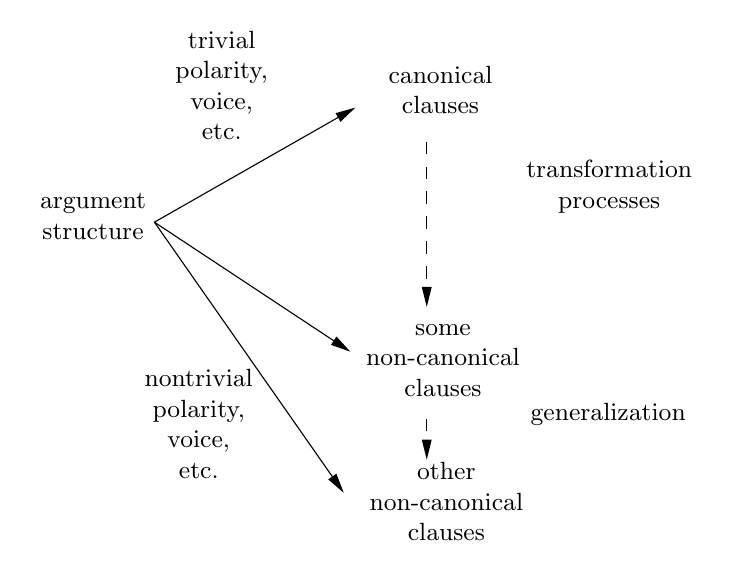
\begin{tikzpicture}[x=0.75pt,y=0.75pt,yscale=-0.8,xscale=0.8]
        \small
        %uncomment if require: \path (0,386); %set diagram left start at 0, and has height of 386
        
        %Straight Lines [id:da13680161853786577] 
        \draw    (194,152.81) -- (313.26,84.8) ;
        \draw [shift={(315,83.81)}, rotate = 150.31] [fill={rgb, 255:red, 0; green, 0; blue, 0 }  ][line width=0.08]  [draw opacity=0] (12,-3) -- (0,0) -- (12,3) -- cycle    ;
        %Straight Lines [id:da16837784710650316] 
        \draw    (194,152.81) -- (310.33,229.71) ;
        \draw [shift={(312,230.81)}, rotate = 213.47] [fill={rgb, 255:red, 0; green, 0; blue, 0 }  ][line width=0.08]  [draw opacity=0] (12,-3) -- (0,0) -- (12,3) -- cycle    ;
        %Straight Lines [id:da07747924239146564] 
        \draw    (194,152.81) -- (306.85,314.17) ;
        \draw [shift={(308,315.81)}, rotate = 235.03] [fill={rgb, 255:red, 0; green, 0; blue, 0 }  ][line width=0.08]  [draw opacity=0] (12,-3) -- (0,0) -- (12,3) -- cycle    ;
        %Straight Lines [id:da42303822011922976] 
        \draw  [dash pattern={on 4.5pt off 4.5pt}]  (358,201.81) -- (358,98.15) ;
        \draw [shift={(358,203.81)}, rotate = 270] [fill={rgb, 255:red, 0; green, 0; blue, 0 }  ][line width=0.08]  [draw opacity=0] (12,-3) -- (0,0) -- (12,3) -- cycle    ;
        %Straight Lines [id:da4793554387643766] 
        \draw  [dash pattern={on 4.5pt off 4.5pt}]  (358,293.81) -- (358,266.81) ;
        \draw [shift={(358,295.81)}, rotate = 270] [fill={rgb, 255:red, 0; green, 0; blue, 0 }  ][line width=0.08]  [draw opacity=0] (12,-3) -- (0,0) -- (12,3) -- cycle    ;
        
        % Text Node
        \draw (118,134) node [anchor=north west][inner sep=0.75pt]   [align=left] {\begin{minipage}[lt]{44.93pt}\setlength\topsep{0pt}
        \begin{center}
        argument\\structure
        \end{center}
        
        \end{minipage}};
        % Text Node
        \draw (200,36) node [anchor=north west][inner sep=0.75pt]   [align=left] {\begin{minipage}[lt]{39.53pt}\setlength\topsep{0pt}
        \begin{center}
        trivial\\polarity,\\voice,\\etc. 
        \end{center}
        
        \end{minipage}};
        % Text Node
        \draw (328,57) node [anchor=north west][inner sep=0.75pt]   [align=left] {\begin{minipage}[lt]{44.05pt}\setlength\topsep{0pt}
        \begin{center}
        canonical\\clauses
        \end{center}
        
        \end{minipage}};
        % Text Node
        \draw (313,213) node [anchor=north west][inner sep=0.75pt]   [align=left] {\begin{minipage}[lt]{63.87pt}\setlength\topsep{0pt}
        \begin{center}
        some\\non-canonical\\clauses
        \end{center}
        
        \end{minipage}};
        % Text Node
        \draw (315,296) node [anchor=north west][inner sep=0.75pt]   [align=left] {\begin{minipage}[lt]{63.87pt}\setlength\topsep{0pt}
        \begin{center}
        other\\non-canonical\\clauses
        \end{center}
        
        \end{minipage}};
        % Text Node
        \draw (181,240) node [anchor=north west][inner sep=0.75pt]   [align=left] {\begin{minipage}[lt]{45.76pt}\setlength\topsep{0pt}
        \begin{center}
        nontrivial\\polarity,\\voice,\\etc. 
        \end{center}
        
        \end{minipage}};
        % Text Node
        \draw (409,114) node [anchor=north west][inner sep=0.75pt]   [align=left] {\begin{minipage}[lt]{68.79pt}\setlength\topsep{0pt}
        \begin{center}
        transformation\\processes
        \end{center}
        
        \end{minipage}};
        % Text Node
        \draw (412,260) node [anchor=north west][inner sep=0.75pt]   [align=left] {\begin{minipage}[lt]{64.45pt}\setlength\topsep{0pt}
        \begin{center}
        generalization
        \end{center}
        
        \end{minipage}};
        
        
        \end{tikzpicture}
    \caption{What is a transformation rule}
    \label{fig:transformation-rule}        
\end{figure}

\subsection{The nominal system}

\subsection{The verbal system}

\subsubsection{Verb conjugation}\label{sec:conjugation-form}

Different people use the term \term{verb forms} -- and count them -- in different ways.
The most generous -- and the most syntactically relevant -- way 
is to view the realization of every possible CP-TP-\vP{} projection 
as a form of the main verb -- the verb root at the core of the CP-TP-\vP{} domains.
This results in a paradigm in traditional grammar, 
essentially the traditional way to enumerate Latin verb forms 
(``the indicative active present second person form of a verb is \dots'').

The problem with this approach is sometimes two cells in the paradigm are always identical.
In this way, morphosyntactically there are indeed two different paradigm cells,
but morphophonologically there is only one verb form.
Take English as an example: 
a traditional grammar may say 
``the present subjunctive first person singular of English \form{take} is \form{take}''. 
The problem here is the present subjunctive first person singular \emph{clause}
always contains the same form of the \emph{verb}
with a present indicative first person singular clause,
so it makes no sense to talk about ``the present subjunctive first person singular \emph{verb form}''.
A linguist stingy with the number of verb forms 
may then stipulate that conjugation forms are literally about \emph{forms},
and thus there is no such thing as ``the subjunctive form'' of English verbs,
because in subject \emph{clauses}, 
the main verb always has the same form as the infinitive
\citep[\citepage{76}]{cgel}.

Another problem with this approach occurs 
when dealing with languages like Japanese.
There are so many suffix slots,
and the boundaries between suffixes are relatively clear,
so the paradigm is too big to be displayed as a whole
and too regular to be enumerated cell by cell.
In this case, recording suffixes may be a better choice.

The analysis of conjugation forms of the verb, theoretically speaking,
is more about vocabulary insertion and readjustment rules,
instead of the syntax proper.
This is an instance of the \emph{separation principle}:
morphophonological features can be separated from morphosyntactic features
\citep{embick2000features}.
Distinguishing between verb forms and clause categories isn't just a game about wording:
in periphrastic conjugation,
we have auxiliary verb(s) plus a non-finite verb form,
but here the non-finite verb form is just the spellout of several features together with the verb root 
and is definitely not thea head of a non-finite \emph{clause}:
what we have here is one clause, not clause embedding.
Thus it makes no sense to say ``we use a non-finite verb form in a periphrastic construction'',
because finiteness is a category of a clause,
and here is no clause combining.
This is also relevant for surface-oriented descriptive linguistics:
\citet[\citepage{74,83}]{cgel} rejects the notion of the \term{infinitive form} of the verb,
and replace the term by \term{default form},
because the so-called infinitive form also appears in the subjunctive mood
or the imperative mood. 
Despite this, to respect the tradition, 
I will still use the term \term{non-finite verbs} 
or wordings like ``the perfect passives are formed by attaching forms of copula to the perfect participle''.

The generous paradigm-cell-as-verb-form approach fortunately works in Latin 
because Latin is morphologically rich
and thanks to historical changes,
the boundaries between suffixes marking each grammatical category 
are already vague enough, so the Japanese School Grammar approach is also not applicable. 
So it does make sense to talk about 
``the indicative active perfect second person singular form'' of a verb.
Similarly, we also talk about non-finite verb forms (\prettyref{sec:non-finite-abs}),
though strictly speaking, finiteness is a category of the clause.

\subsubsection{Argument structure}\label{sec:a-position}

\paragraph{Three aspects of verb valency} 
To achieve a disciplined analysis of verb valency, 
we may adopt a multiple-step analysis of A-positions
(i.e. the positions in the syntactic frame of a verb):
at least two steps -- the \vP{} step and the TP step 
-- are to be distinguished in syntax, 
apart from the purely semantic verb classification.
Thus, a three-step model -- 
the steps being pure semantics
(``Manipulator'' or ``Target'', i.e. those listed in \citet{dixon2005semantic}), 
coarse-grained argument semantic roles with syntactic significance 
\citep[\citesec{4.2}]{cgel}, 
and clausal dependent positions directly analyzable using constituent order or case
(subject, object, etc.) -- 
is needed to fully cover verb valency.
Note that in this note it's \emph{not} assumed that 
a completely transparent mapping exists 
from semantics to syntax.
In English, for example, \form{I like this} 
(\form{this} represents an event)
is semantically complement-taking 
but involves no complement clause construction syntactically;
and it's possible to leave out a semantic argument in the syntactic frame of a verb.

\paragraph{Necessity to talk about ``syntactic''  semantic roles} 
In practice usually we will conflate these ``syntactic'' semantic roles 
and more apparent clausal dependent slots 
and compare these syntactic concepts 
-- essentially A-positions -- with purely semantic concepts.
This approach is bound to be fruitful, 
since no one-to-one relation exists between A-positions and pure semantic roles.%
\footnote{
    Similar things happen in event structure: 
    A Secondary verb is different from, say, an auxiliary verb in the verbal system
    in the eye of syntax 
    and at the syntax-semantic interface:
    the lexical verb \form{start}, for example, 
    introduces a new event besides the event that the agent is start to do, 
    while an inchoative aspect, 
    if in the grammatical aspect region and not the lexical aspect region,
    reflects the speaker's attitude
    (possibly by shifting the time referred to 
    to the initial part of the whole situation),
    but they are of course equivalent to each other,
    although their interpretations 
    immediately at the syntax-semantic interface 
    are different.
}
But it's still not enough: in passivization, 
while the agent argument still occupies a higher position,
it receives an inherent case (quite similar to how DPs are licensed by prepositions)
and is thus unable to move to the subject position.
This demonstrates the necessity to distinguish \emph{two} layers of grammatical relations in A-positions.
Dixon refers to them as ``deep'' and ``surface'' argument slots, 
and this notation is also taken in this note.

On the other hand it may be tempting to conflate 
``syntactic'' semantic roles with purely semantic roles 
and compare them with apparently analyzable clausal dependent positions 
like subject, object, etc.
Indeed, ``syntactic'' semantic roles -- \term{thematic roles} in generative syntax -- 
are first obtained with coarse-graining of 
various verb-specific semantic roles,
and then we find a strong correlation between thematic roles 
and their deep syntactic positions, 
and this gives rise to the Uniformity of Theta-Assignment Hypothesis (UTAH).
So in principle conflating the two should have no problem
as long as we choose the correct coarse graining method.
The problem however is this often goes against the tradition:
we often say \form{the stick} in \form{I hit the wall with the stick} and 
\form{I hit the stick to the wall}
have the same purely semantic role (the thing manipulated by the agent),
but their syntactic semantic roles are completely different
(instrument v.s. patient);
this difference is reflected in semantics, 
since we would say the second example focuses on the stick,
but still people usually think this difference is kind of small.

Some alternations, like the alternation of the clausal complement position of 
the experiencer roles in  
\form{he fears the police} and \form{the police frightens him},
are hard to locate: 
they may be different in the \vP{} step,
or they are the same in the \vP{} step but something else decides 
which argument becomes the subject.
But anyway, the above discussion means it's necessary to create 
a layer of ``syntactic'' semantic roles
between purely semantic concepts and surface clausal slots.

\paragraph{A-positions in an accusative language} 
Assignment of the accusative case is said to be done within the \vP region.
Then comes the TP step, in which
usually the highest argument position in the \vP{} step -- also the most agentive one --
becomes SpecTP, 
which is better known as the subject.

\paragraph{Generalized semantic roles and ambiguity in terminology} 
The tendency to use ``surface-orientated terms'' in typology 
somehow makes the terminology concerning the 
above three steps in syntactic derivation confusing.\footnote{
    Here \term{derivational} means what it means in modern generative grammar, 
    that grammatical structures are built by successive applications of (possibly internal) Merge.
    It \emph{doesn't} mean \emph{transformational operations}
    in early versions of generative grammar.
}
So-called generalized semantic roles like S, A, P, etc.
are used to refer to labels in all the three steps, 
and when they are used in describing the last two steps,
they are \emph{syntactic} labels, despite the name. 
The following example demonstrates this chaos.
Consider an unaccusative verb in an accusative language,
like \form{hurt} in \form{my fingers hurt}.\footnote{
    Note that unaccusativity has nothing to do with alignment:
    we can have unaccusative verbs in a typical accusative language, like English.
} 
In the argument structure of an unaccusative verb,
no agentive argument is present,
so we may say there is no A argument. 
The deep P argument becomes the surface S argument,
which then may be called an A argument since in accusative languages S=A.
Similarly the meaning of the term \term{semantic role}
needs to be inferred from the context.
This is also an example why we need to tell deep argument positions (i.e. positions in \vP{})
from surface argument positions (positions after TP or even CP is built).

\paragraph{Ergativity and split of grammatical relation labels}
It should be noted that labels for A-positions, like \term{subject},
are bundles of several syntactic functions
(in the case of \term{subject}, 
it's the external argument which governs all internal complements, 
the receiver of the nominative case, and, say, SpecDoP, 
where Do or something else is the highest light verb in the \vP{} field).
When these syntactic functions are disassembled with each other, 
the corresponding collective label no longer makes sense.
Thus in a morphological ergative language, 
the ``nominative case receiver'' syntactic function is absent, 
and the A argument of a transitive verb receives an inherent case, 
so the A argument loses the morphological resemblance with the 
S argument for intransitive verbs, 
but it keeps the syntactic functions of 
the highest argument; 
for syntactic ergativity, 
the external argument property is given to the P argument \citep{aldridge2008generative}.
In both cases, grammatical relations condensed into the label \term{subject} 
need to be taken out one by one and redistributed to new collective terms.

\paragraph{Valence changing} From a generative perspective, some languages realize valency changing 
by a series of \vP{} structures, and then the case assignment of the arguments is trivial.
Some languages use non-trivial structural case assignment mechanisms
to achieve valency changing 
(``suppressing the agent argument, 
and leave the nominative probe to find the subject;
the probe then has to choose the patient argument'').
Of course, \vP{} changes in the second type are still there,
which may be a likely source of relevant verb morphology.
Naturally, the second group of languages have more restricted valency changing devices;
this is the case of Latin.

\paragraph{Deponent verbs} 
In the analysis in \citet{embick2000features} 
a verb is deponent if its root is only able to 
appear together with the passive Voice feature. 
When functional heads higher than the roots are realized,
the passive feature -- which may come from the root or from the passive light verb -- 
guides the realization of the person and number categories.
Then since the similarity between unaccusative verbs and passive verbs
(the surface S argument being the deep O argument),
we can expect that
the two may have similar behaviors at least in some languages,
which is already demonstrated by second language acquisition,
which arguably reflects the ``default'' parameter setting of languages \citep{balcom1997happened}.
Latin also has this phenomenon \citep[\citepages{308-309}]{oniga2014latin}.

\paragraph{Documenting complement types}

The traditional practice of Latin grammar research
is to classify clausal complement and adjunct types according to their case marking.
This strategy is also found in modern grammars.
Some introduce clausal complement types just in chapters about case marking 
\citep[\citechap{8}]{jacques2021grammar},
while other grammars, despite giving a brief description of the context of case marking,
spare some time to discuss complement types in the chapters about valency and clause structure 
\citep[\citesec{3.4}, \citechap{19}, \citechap{22}]{forker2020grammar}.
From a \ac{tag} perspective (\prettyref{sec:theoretical-orientation}), 
the two extremes are different in how they treat function labels:
in the former, the function label of a construction appears together with its category label on the root node,
while in the latter, the function is described separately from the form of what fills that position.
The former is more bottom-up, 
while the latter is more top-down.
The choice between the two, however, is usually language-dependent:
grammars for analytic languages, of course, have to lean even further to the 
``complement type as clause slot'' extreme 
and away from the ``complement type as case-form context'' extreme.
\citet{allen1903allen} uses a hybrid method:
the discussion about case marking (\citesec{39}) is separated from 
the discussion about complement and adjunct types (\citesec{338}),
so the top-down approach seems to be adopted,
but the latter is still arranged in terms of case.
This arises both from the distinct features of Latin and the intended readers:
the relation between complement types and cases is regular enough in Latin,
and what is most important for Latinists is to understand, at least sketchily, ancient writings, 
so a parsing-oriented grammar is much handier.

\subsubsection{Clause combining}

It's hard to draw a line between coordination and asymmetric (i.e. subordinating) clause linking 
(like concessive clauses).
Theoretically, this is because any clause combining construction follows the X-bar scheme:
one clause is the Specifier, 
and another clause is the Complement,
and certain asymmetry has to be introduced.
In English, the FANBOYS 
-- \form{for}, \form{and}, \form{nor}, \form{but}, 
\form{or}, \form{yet}, \form{so} -- are usually regarded as coordinating conjunctions.
But what's the essential difference between \form{although} and \form{but}?

On the other hand, adverbial clause constructions 
are uncontroversially asymmetric and can in theory be distinguished from clause linking:
in clause linking, the less important clause 
is base-generated in one Specifier position in the CP layer of the main clause,
so the two combined units are of roughly the same structure,
while adverbial clauses appear in the TP layer,
so the two combined units are of different structures:
the adverbial clause is a CP,
while the main clause, when the adverbial clause enters derivation,
is a TP.
Complement clauses, on the other hand, are first introduced in the \vP{} layer:
they are TPs or CPs,
while the main clause, when complement clauses enter the derivation,
are \vP s.
But there are still certain subtleties regarding the boundaries of \vP{}, TP, and CP.

Relative clauses are introduced in DPs, 
so the probability to confuse a relative clause construction 
with a complement clause construction is small -- but still not zero.
It can be expected that \form{I like the man dancing} and \form{I like the dancing man} 
are realized in quite similar ways.
Besides, some languages lack prototypical complement clause constructions 
but have complementation strategies.
That is, when they talk about \form{I like the dancing man},
a speaker of such a language may be implying that he or she actually likes the man's dancing,
though not the man's personality.
Now comes the question:
when there are vague evidences indicating the grammaticalization of this construction,
should we now claim the language has already developed a complement clause construction?

It's still possible to do the same thing 
-- largely symmetric coordination and certainly asymmetric subordination -- 
completely with \vP s.
The former results in clause chaining \citep{nonato2014clause},
while the latter results in serial verb constructions.
These construction types, however, are absent in Latin, and I will not go deep into them in this note.

\subsection{Constituent order and information packaging}

The fact that fine-grained constituency relation exists in Latin 
is probably not surprising because
even the most non-configurational languages show configurationality 
under scrutiny
\citep[among others]{niedzielski2017clausal,morris2018evidence,legate2002warlpiri}
and therefore a thorough disruption 
of the existing framework of generative syntax seems unnecessary.%
\footnote{
    There is still some left controversies over 
    whether prototypical non-configurational languages 
    have a \emph{different} constituent structure,
    like, say, the structure in pronominal argument hypothesis (PAH),
    in which argument positions are filled by pronominals 
    in the nucleus clause,
    while the \acs{np} ``arguments'' are base-generated topics 
    linked to the argument positions not by movement.
    Even though this seems plausible, 
    \cite{legate2002warlpiri} rejects the hypothesis.
}
Still, even though we know mainstream generative (constituency-based, 
though the introduction of movements and the structure of Cinque hierarchy
gives it certain flavor of dependency grammars) approaches make perfect sense for Latin,
a systematic and thorough description of Latin grammar 
would be better carried out in a dependency-relation based or \acs{blt}-based way.
This is of course mostly notational change:
for example, we only recognize the most ``salient'' types of constituents 
like \acs{np}s and clauses as constituents in our description,
and the existence of fine-grained functional projections is covered by 
additional information like the ``height'' or ``closeness'' of dependency arcs
corresponding to these functional projections
(\prettyref{sec:theoretical-orientation}).

}
